\documentclass[conference]{IEEEtran}
\usepackage[top=2.5 cm, bottom=2.5 cm, left=2.0 cm, right=2.0 cm]{geometry}
\geometry{letterpaper}
\usepackage[parfill]{parskip}
\usepackage{graphicx}
\usepackage{amsmath}
\usepackage{amssymb}
\usepackage{comment}
\usepackage{epstopdf}
\usepackage{subfigure}
\usepackage{extarrows}
%\usepackage{minted}
\usepackage{tensor}
\usepackage{float}
%\usemintedstyle{vs}
\usepackage{kbordermatrix}
\usepackage{my_acronyms}

\DeclareGraphicsRule{.tif}{png}{.png}{`convert #1 `dirname #1`/`basename #1 .tif`.png}



\title{Realtime 6-DOF SLAM for a Quadrotor Helicopter}

%  \author{\IEEEauthorblockN{Stephen Chaves}
%   \and
%   \IEEEauthorblockN{Schuyler Cohen}
%   \and
%   \IEEEauthorblockN{Patrick O'Keefe}
%   \and
%   \IEEEauthorblockN{Paul Ozog}
%  \IEEEauthorblockA{\IEEEauthorrefmark{1}School of Electrical and Computer Engineering\\
%    Georgia Institute of Technology, Atlanta, Georgia 30 332--0250\\
%    Email: mshell@ece.gatech.edu}
% }


 \author{\IEEEauthorblockN{Stephen Chaves\ \ \ \ \  Schuyler Cohen\ \ \ \ \  Patrick
     O'Keefe\ \ \ \ \  Paul Ozog}\\
   \IEEEauthorblockA{University of Michigan}
}

% \author{\IEEEauthorblockN{Michael Shell\IEEEauthorre fmark{1}, Homer Simpson\IEEEauthorrefmark{2}, James K irk\IEEEauthorrefmark{3}, Montgomery Scott\IEEEauthorrefmark{3} and Eldon Tyrell\IEEEauthorrefmark{4}} \IEEEauthorblockA{\IEEEauthorrefmark{1}School of Ele ctrical and Computer Engineering\\
% Georgia Institute of Technology, Atlanta, Georgia 30 332--0250\\
% Email: mshell@ece.gatech.edu} \IEEEauthorblockA{\IEEEauthorrefmark{2}Twentieth Cen tury Fox, Springfield, USA\\
% Email: homer@thesimpsons.com} \IEEEauthorblockA{\IEEEauthorrefmark{3}Starfleet Aca demy, San Francisco, California 96678-2391\\ Telephone: (800) 555--1212, Fax: (888) 555--1212} \IEEEauthorblockA{\IEEEauthorrefmark{4}Tyrell Inc.,
% 123 Replicant Street, Los Angeles, California 90210 --4321}}

\begin{document}
\maketitle



\begin{abstract}

  This paper presents a realtime implementation of a \ac{SLAM} framework for a quadrotor
  helicopter.  The framework features a front-end interface to the helicopter and a
  back-end solver of the graph representation of the robot and its environment. The
  back-end implements techniques from incremental Smoothing and Mapping (iSAM) in order to
  solve the graph in real time and provide instananeous visualization of the robot
  trajectory and landmark positions. iSAM incrementally updates the information matrix
  factorization, providing significant time savings over other \ac{SLAM} solvers. The speedups
  resulting from iSAM allow the 6-\ac{DOF} \ac{SLAM} problem to be solved in realtime on a
  consumer-grade computer. Our software implementation was successfully tested in simulation
  and using an AR.Drone quadrotor helicopter.

\end{abstract}






\section{Introduction}
\label{sec:introduction}


\ac{SLAM} problems present many computational challenges, most of which stem from the
large number of observations and states which must be reconciled. Least-squares approaches
are particularly affected by these problems; naive implementations are too slow to be used
in realtime scenarios. Work from \cite{dellaert2005square} was the basis for incremental
approaches such as iSAM \cite{Kaess08tro}, which allow least-squares based methods to run
in realtime. For this work, we seek to implement and apply these techniques to a quadrotor
helicopter.


For robotics reseach, quadrotor helicopters are a popular platform because of their
maneuverability, stability, and relatively low mechanical complexity. In
\cite{achtelik2008autonomous}, an \ac{EKF} was successfully used for realtime \ac{SLAM} on
a quadrotor platform, which avoids the problems associated with least-squares altogether. Very
recent work \cite{ghadiok2011autonomous} has allowed for fully autonomous quadrotors with
SLAM capabilities. However, the sensor suite on their platform is very expensive.


In this paper, we present a modular implementation of a \ac{SLAM} system. We then discuss
optimizations to our SLAM algorithm -- inspired by iSAM -- which allow for realtime
operation. This paper also covers our generic observation and motion models for 6-\ac{DOF}
systems. Finally, we apply our system to a number of simulations and real-world datasets
including a quadrotor helicopter.



\section{System Architecture}
\label{sec:systemarchitecture}

% Steve's Section

The architecture of our \ac{SLAM} software was developed with modularity and versatility
in mind.  As a result, our software consists of two subsystems: a
front-end that interfaces with the robot and creates nodes and factors from
odometry and landmark observations, and a back-end that solves the \ac{SLAM} problem from
a graph generated from these nodes and factors.

In our framework, each robot node is a six dimensional pose and each landmark node is a
three dimensional position. These poses and positions make up the state vector solved by
the back-end. The factors represent constraints between two unknowns or a constraint for a
single unknown. From these factors we can extract Jacobians and residuals associated with
the underlying optimization problem. Describing a system with nodes and factors creates
an elegant representation of any least-squares problem. This representation was
successfully applied to the \ac{SLAM} problem in~\cite{dellaert2005square}.


Our software system consists of multiple processes. In order to pass information between
them, we employ the Lightweight Communications and Marshalling (LCM)
library~\cite{huang2010}. One of the main benefits of using LCM is the ability to record
and playback the messages sent between processes. This tool allows us to keep a record of
the experiments we performed and evaluate different algorithms on the same
real-world dataset. The front-end also uses LCM to receive data from the robot and to send
it motion commands.

By designing the software as a modular framework, the back-end is a generic solver for any
graph-based \ac{SLAM} problem. Thus, the back-end can be easily transferred between
\ac{SLAM} applications. Only the front-end is specific to the application, and it is
responsible for data association. The back-end solver we implemented is inspired by iSAM
(discussed in Section~\ref{sec:incrementalsmoothingandmapping}). Moreover, the modularity
of our system allows us to test different least-squares solvers without altering the
front-end.

\section{Incremental Smoothing and Mapping}
\label{sec:incrementalsmoothingandmapping}

%Pat's section

Incremental smoothing and mapping is a relatively recent approach to solving the
full \ac{SLAM} problem~\cite{Kaess08tro}.  The full \ac{SLAM} problem, in contrast to the
online \ac{SLAM} problem, recovers the full posterior of the robot trajectory and landmark
positions instead of just the current robot pose and landmark
positions~\cite{thrun2005probabilistic}.

In standard least-squares \ac{SLAM}, we solve a system of equations such as
\begin{align*}
  \Delta x' &= \underset{\Delta x}{\operatorname{argmin}} (J\Delta x - r)^{\text{T}}
\Sigma^{-1} (J\Delta x - r) \\
  &= \underset{\Delta x}{\operatorname{argmin}} \| J\Delta x - r \|^2_{\Sigma}
\end{align*}
where $x$ is the state vector that contains all robot poses and
landmark positions, $J$ is the Jacobian of the observation model that
predicts measurements given the state vector, $\Delta x$ is the
deviation of $x$ from the linearization point, and $r$ is the residual
of observations versus the predicted measurements. The minimizing
solution results in the standard normal equations given by
\[
(J^{\text{T}} \Sigma^{-1} J) \Delta x = J^{\text{T}} \Sigma^{-1}r
\]
This is solved via the Cholesky decomposition of the information matrix,
$J^{\text{T}}\Sigma^{-1}J$.

iSAM makes a change to this problem formulation by considering the Cholesky decomposition
of $\Sigma^{-1}$ -- written as $\Sigma^{-\text{T}/2}$ to denote the upper triangular
result of the decomposition --  and rewriting the least squares problem as
\begin{align*}
    \Delta x' &= \underset{\Delta x}{\operatorname{argmin}} (J\Delta x - r)^{\text{T}}
\Sigma^{-1/2}\Sigma^{-\text{T}/2} (J\Delta x - r) \\
  &= \underset{\Delta x}{\operatorname{argmin}} \| \Sigma^{-\text{T}/2}(J\Delta x - r)
  \|^2\\
&= \underset{\Delta x}{\operatorname{argmin}} \| (A\Delta x - b)\|^2
\end{align*}
where
\begin{align*}
  A &= \Sigma^{-\text{T}/2}J \\
  b &= \Sigma^{-\text{T}/2}r
\end{align*}
This allows us to solve $A\Delta x = b$ by applying QR factorization directly to $A$. This
is advantageous because it avoids the squaring of the matrix condition number that is
associated with the normal equation form. Moreover, there is the nice property that the
$R$ that results from the QR decomposition of $A$ is equivalent to the upper triangular
term in the Cholesky decomposition of $A^{\text{T}}A$ if A is real~\cite{Kaess08tro}.

iSAM recovers the posterior by doing fast incremental updates to the factorization of $A$.
This means that calculations are only performed on elements that are actually affected by
new measurements. We can get away with this because we often have a very good estimate of
the state vector so doing a full batch re-linearization and solution at each step wastes
calculations because most elements of $\Delta x$ will be close to zero. However, iSAM
periodically performs a full batch solution in order to compensate for accumulated
linearization errors. Over time, loop closures greatly decrease the sparsity of the matrix
factorization, so variable reordering is performed during each batch solution step.

\subsection{Givens Rotations}
\label{sub:givensrotations}

When a new measurement row is added to $A$, we can incrementally update $R$
instead of performing the entire QR decomposition again. This can be achieved with Givens
rotations.

Givens rotations are a way to introduce a zero at a specified point in a matrix by
premultiplying by a matrix $G$ of the form


\[
G(i, k, \theta) =
\kbordermatrix{  & & &i& &k & & \\
 & 1   & \cdots &    0   & \cdots &    0   & \cdots &    0   \\
 & \vdots & \ddots & \vdots &        & \vdots &        & \vdots \\
i & 0   & \cdots &    c   & \cdots &    -s   & \cdots &    0   \\
 & \vdots &        & \vdots & \ddots & \vdots &        & \vdots \\
k & 0   & \cdots &   s   & \cdots &    c   & \cdots &    0   \\
 & \vdots &        & \vdots &        & \vdots & \ddots & \vdots \\
 & 0   & \cdots &    0   & \cdots &    0   & \cdots &    1
       }
\] 

where $c = \cos{(\theta)}$ and $s = \sin{(\theta)}$ for some $\theta$. We follow the
algorithms in Golub and Van Loan's \emph{Matrix Computations} to find $c$ and $s$ to
zero a particular element in a matrix~\cite{golub1996matrix}.

The $R$ term that results from the QR decomposition of $A$ is upper triangular by
definition. When a new measurement occurs, new rows need to be added to $A$. Here, we
append them to $R$, which is then no longer upper-triangular. A series of Givens rotations
is applied to the elements that are below the diagonal. This is called triangularization,
and once the below-diagonal elements have been removed via the rotations, the resulting
upper-triangular matrix is equivalent to the QR decomposition of the full $A$
matrix~\cite{golub1996matrix}. The same series of rotations needs to be applied to our
right-hand side term, $b$.

After the rotations have been performed, the system can be solved with simple back-substitution.

\begin{figure*}[t]
  \begin{center}
    \subfigure[] {
    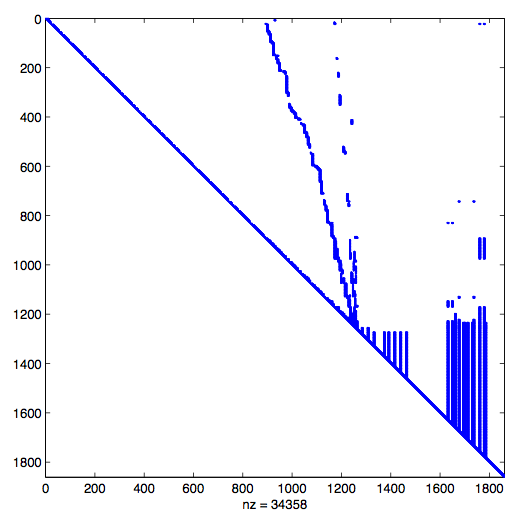
\includegraphics[width=2.5in]{images/reorder32}
    \label{fig:images/reorder32}}
    \subfigure[] {
    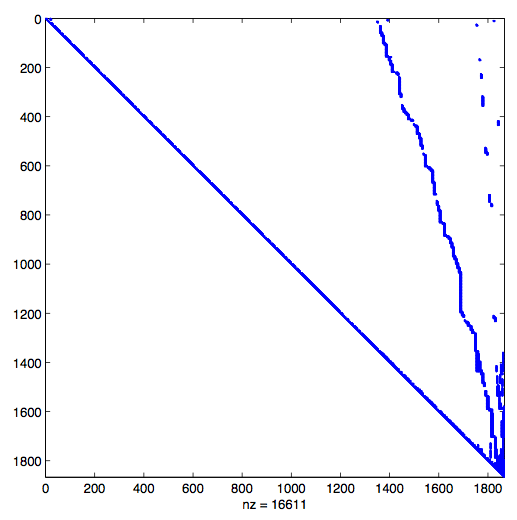
\includegraphics[width=2.5in]{images/reorder33}
    \label{fig:images/reorder33}}
    \caption{The factorization of the $A$ matrix after 300 time steps of simulated data
      that includes loop closures. (a) Before variable reordering, the loop closures
      introduce many non-zero elements. (b) After variable reordering, we have a much more
    sparse factorization. Over 50\% of the non-zero elements were removed.}
    \label{fig:reorder}
  \end{center}
\end{figure*}

\subsection{Variable Reordering}
\label{sub:variablereordering}

When a robot closes a loop, a correlation is introduced between the current pose and a
previously observed landmark. This landmark is connected to earlier poses in the
trajectory as well. These correlations greatly increase the number of non-zero elements in
the matrix factorization which in turn increases the computational complexity of updating
and solving the system. Figure \ref{fig:images/reorder32} shows the large swaths of
non-zero elements that are introduced during loop closures. 

In order to avoid this problem, we can perform variable reordering. This is essentially a
permutation of the columns of $A$ where columns that belong to the same node in the \ac{SLAM}
graph are kept together. This new order influences the variable elimination, which
has a profound effect on the sparsity of the factorization. Figure
\ref{fig:images/reorder33} shows the result of applying variable reordering to simulated
data that has experienced several loop closures.

The best column variable ordering is NP hard, and iSAM uses COLAMD as a heuristic to
assist in the process~\cite{davis2004column}. Our implementation uses a simplified
heuristic that counts the number of connected nodes in the graph. It is not the minimum
degree ordering, but we have found it to be more than adequate in our tests. Figure
\ref{fig:reorder} is an example of the application of our simplified heuristic.

\section{Back-end Motion and Observation Models}
\label{sec:backendModels}

Because of the relative complexity of 6-\ac{DOF} coordinate transforms, we used a notation
that allows us to abstract away the linear algebra operations necessary for the nonlinear
motion and observation models. To achieve this, we adopt the notation
from~\cite{rsmith-1990a,reustice-phdthesis} to describe three particular spatial
relationships of 6-\ac{DOF} coordinate frames: {\it compound, inverse}, and {\it
  composite}. These relationships are used throughout our system.


\subsection{6-\ac{DOF} Spatial Relationships}
\label{sec:6dof}
% Paul's section


Let ${\bf x}_{ij} = \begin{bmatrix}
  {\bf t}_{ij}^i & {\boldsymbol \Theta}_{ij}\\
\end{bmatrix}^\top$ be a vector in $\mathbb{R}^6$ describing the
relative pose of frame $j$ with respect to frame $i$.  ${\bf
  t}_{ij}^i$ is the $3\times 1$ translation vector from frame $i$ to
frame $j$ as expressed in frame $i$.  ${\boldsymbol \Theta}_{ij}$ is
the $3 \times 1$ vector describing the Euler angles of the $x$, $y$,
and $z$ axes.  We define the function $(\text{rotxyz}: \mathbb{R}^3
\rightarrow \mathbb{R}^{3\times3})$ that maps a vector of Euler angles to
a rotation matrix as follows:
\begin{eqnarray*}
  R_j^i & = & \text{rotxyz}({\boldsymbol \Theta}_{ij})
\end{eqnarray*}
where $R_j^i$ is the matrix that rotates frame $j$ into frame $i$.

These definitions allow us to describe the transformation matrix
that uniquely relates homogeneous 3D points in frame $j$ to homogeneous
points in frame $i$ as:
\begin{eqnarray*}
  H_{j}^i & = & \begin{bmatrix}
    R_j^i & {\bf t}_{ij}^i\\
    {\bf 0} & 1
  \end{bmatrix}
\end{eqnarray*}
Note that given $H_j^i$, we can easily compute ${\bf x}_{ij}$ and vice
versa using APRIL's \texttt{LinAlg} Java package.

\subsubsection{Compounding Operation}
\label{sub:compoundingoperation}

Let the $\oplus$ operator describe the spatial relationship between
two frames arranged ``head-to-tail'':
\begin{eqnarray*}
  {\bf x}_{ik} & = & {\bf x}_{ij} \oplus {\bf x}_{jk} 
\end{eqnarray*}
${\bf x}_{ik}$ can be computed from recovering the $6 \times 1$ vector
corresponding to the matrix
\begin{eqnarray*}
  H_k^i & = & H_j^i H_k^j
\end{eqnarray*}

% For example, for the compounding operation, our \ac{SLAM} back-end takes $i$
% to denote the world frame.  $j$ and $k$ denote the frame of the robot
% at the previous and current timesteps, respectively.  This effectively
% acts as a motion model that predicts the global pose of a robot in
% 6-\ac{DOF} given the odometry at every timestep.

The Jacobian of the compounding operation $J_\oplus$ is given
in~\cite{reustice-phdthesis}.  Using this matrix, we can compute the covariance of ${\bf
  x}_{ik}$ as the covariance projection

\begin{eqnarray*}
  \Sigma({\bf x}_{ij}) & = & J_\oplus \begin{bmatrix}
    \Sigma({\bf x}_{ik}) & \Sigma({\bf x}_{ij}, {\bf x}_{kj})\\
    \Sigma({\bf x}_{kj}, {\bf x}_{ij}) & \Sigma({\bf x}_{kj})\\
  \end{bmatrix} J_\oplus^\top
\end{eqnarray*}

\subsubsection{Inverse Operation}
\label{sub:inverseoperation}
Let the $\ominus$ operator describe the inverse of a relative pose
vector:
\begin{eqnarray*}
  {\bf x}_{ji} & = & \ominus {\bf x}_{ij}
\end{eqnarray*}
This operation is computed from the transformation matrix
\begin{eqnarray*}
  H_i^j & = & \left(H_j^i\right)^{-1} \\
  & = & \begin{bmatrix}
    \left( R_j^i \right)^\top & -\left( R_j^i \right)^\top {\bf t}_{ij}^i\\
    {\bf 0} & 1
  \end{bmatrix}
\end{eqnarray*}
The first-order covariance projection of this operation is
\begin{eqnarray*}
  \Sigma({\bf x}_{ji}) & = & J_\ominus \Sigma({\bf x}_{ij}) J_\ominus^\top
\end{eqnarray*}
where the closed-form expression for the Jacobian is given
in~\cite{reustice-phdthesis}.

\subsubsection{Composition Operation}
\label{sub:compositionoperation}
We define the composite operation on two frames related
``tail-to-tail'' using the compounding and inverse operations:
\begin{eqnarray*}
  {\bf x}_{jk} & = & \ominus {\bf x}_{ij} \oplus {\bf x}_{ik}
\end{eqnarray*}
where the Jacobian of this relationship is 
\begin{eqnarray*}
  \tensor[_\ominus]{J}{_\oplus} & = & J_\oplus \begin{bmatrix}
    J_\ominus & 0_{6 \times 6}\\
    0_{6 \times 6} & I_{6 \times 6}\\
  \end{bmatrix}
\end{eqnarray*}
and thus the first-order covariance projection of the composite
operation is
\begin{eqnarray*}
  \Sigma({\bf x}_{jk}) & = & \tensor[_\ominus]{J}{_\oplus} \begin{bmatrix}
    \Sigma({\bf x}_{ij}) & \Sigma({\bf x}_{ij}, {\bf x}_{ik})\\
    \Sigma({\bf x}_{ik}, {\bf x}_{ij}) & \Sigma({\bf x}_{ik})\\
  \end{bmatrix} \tensor[_\ominus]{J}{_\oplus^\top}
\end{eqnarray*}
% An example application of this composite operation is to estimate the
% odometry of a robot between two successive timesteps (given the
% current and previous poses of the robot in the global frame).  In this
% case, $i$ is the global frame, $j$ is the frame of the robot at the
% previous timestep, and $k$ is the robot frame at the current timestep.
% ${\bf x}_{jk}$ is then the predicted odometry between frame $j$ and
% frame $k$.



\subsection{Node Initialization}
\label{sub:nodeinitializationandedgeresiduals}
Every timestep in which the robot moves or a new feature is observed, a new node is created
and initialized.  To initialize a node means to assign that node a pose (for robot poses)
or a point (for landmarks) in the global frame.  This is computed by the measurement
that relates the new node to a previous node.  To initialize a node without connecting to
a previously created node is a referred to as adding a ``prior.''

For the following sections, let $g$ represent the global frame.  For each node, a
first-order covariance projection can be computed as in Section~\ref{sec:6dof}.

\subsubsection{Pose Nodes}
\label{subs:posenodeinit}

Let frame $i$ correspond to an initialized pose node in the \ac{SLAM} graph.  We observe an
odometry measurement relating frame $i$ and frame $j$.  Then we initialize node $j$ to be
in the global frame with the ``head-to-tail'' operation $ {\hat {\bf x}_{gj}} = {\bf
  x}_{gi} \oplus {\bf x}_{ij} $

\subsubsection{Landmark Nodes}
\label{subs:pointnodeinit}
Given the relative {\it position} of a landmark frame $l$ with respect to robot frame $i$,
we construct a relative {\it pose} vector by setting the orientation of $l$ to be
arbitrary.  Then, the relative {\it position} of the landmark in the global frame is the
translation vector corresponding to $ {\hat {\bf x}}_{gl} = {\bf x}_{gi} \oplus {\bf
 x}_{il} $

\subsection{Factor Computation}
\label{sub:nodeinitializationandedgeresiduals}

To solve the least squares problem described in
Section~\ref{sec:incrementalsmoothingandmapping}, we need to compute an observation model
Jacobian $J$ and residual vector $r$.  Together, these comprise a ``factor'' between two
unknowns in the graph.  In the following section, we describe how these are computed using
the notation from Section~\ref{sec:6dof}.

\subsubsection{Pose-to-Pose Factors}
\label{subs:posenodelinear}
Given two estimates of robot frames $i$ and $j$ (with respect to the global frame), the
predicted relative pose observation is $ {\hat {\bf x}_{ij}} = \ominus {\bf x}_{gi} \oplus
{\bf x}_{gj}$. The Jacobian of this relationship is evaluated as in
Section~\ref{sub:compositionoperation}.  The residual vector is simply the difference
between the predicted ${\hat {\bf x}_{ij}}$ and the observed ${\bf x}_{ij}$.

\subsubsection{Pose-to-Landmark Factors}
\label{subs:pointnodelinear}

If a landmark $l$ is observed from robot frame $i$, then we can predict this measurement
by the ``tail-to-tail'' operation.  We simply assign the orientation of ${\bf x}_{gl}$ to
be arbitrary.  Then, the estimated observation is the translational component of $ {\hat
  {\bf x}}_{il} = \ominus {\bf x}_{gi} \oplus {\bf x}_{gl} $. The residual for the
landmark is the difference between this prediction and what the robot actually measured.

Note that for the computation of this factor's Jacobian, we drop the differentiations with
respect to the orientation of the landmark.  This leaves us with a $3 \times 9$ Jacobian
and $3 \times 3$ positional covariance matrix. 

\section{AprilTag Relative Pose Covariance Estimate}
\label{sec:apriltags}

% Paul's section

We used the AprilTag system throughout our project's experiments and demonstrations for
relative position and orientation.  The accuracy, detection performance, and small memory
footprint made it particularly desirable~\cite{olson2011tags}.

We applied principles of linearized covariance projection to estimate a covariance matrix
for the 6-\ac{DOF} relative pose vector ${\bf x}_{tc}$ that describes the relative pose from
the tag's frame $t$ to the camera's frame $c$.

Denote $f$ as the function that computes the $9 \times 1$ homography vector ${\bf h}$ from
a set of corresponding world points and image points via the Direct Linear Transform (DLT)
algorithm. By linearizing $f$ around a mean input (the observed image point coordinates),
we can compute the $9 \times 9$ covariance matrix $\Sigma({\bf h})$ to a first order
approximation. From there, we project the covariance estimate of $h$ to a pose covariance
by linearizing a function $g$, which maps the homography to ${\bf x}_{tc}$.

For simplicity, we assume that the uncertainty of the world points and the camera
calibration parameters are zero.  Furthermore, we assume negligible lens distortion.  All
differentiations are done numerically.

Under these assumptions, the covariance estimate of the relative pose from tag to camera
is simply
\begin{eqnarray*}
  \Sigma({{\bf x}_{tc}}) & = & J_g J_f \Sigma({\bf u}) J_f^\top J_g^\top
\end{eqnarray*}
where ${\bf u}$ is the $2N \times 1$ vector of $N$ noisy image point coordinates and
$\Sigma({\bf u})$ is the associated covariance matrix.  We assume the feature noise
realizations are independent and isotropic. The diagonal elements of this covariance
matrix are tuned by the user.

The Jacobians are computed by finite difference:
\begin{align*}
  \left[J_f\right]_{ij} &=\frac{\partial f_i}{\partial u_j} \\
  &= \frac{f_i(u_0, u_1, \dots, u_j +
    \epsilon, \dots, u_{2N})}{\epsilon} \\
  & \ \ \  - \frac{f_i(u_0, \dots, u_{2N})}{\epsilon}
\end{align*}
for some small $\epsilon$. One should note that when differentiating $f$, the homography
vectors must have the same sign.  This is not guaranteed in typical Singular Value
Decomposition (SVD) libraries because the sign of the singular vectors may be flipped when
the input matrix is slightly perturbed.

Also, we take $g$ to directly map the homography to ${\bf x}_{tc}$.  The covariance
projections operations referred to in Section~\ref{sec:6dof} are therefore included in $g$.

%Just to see how it looks using both columns
%\begin{figure*}[!t]
%  \begin{center}
%    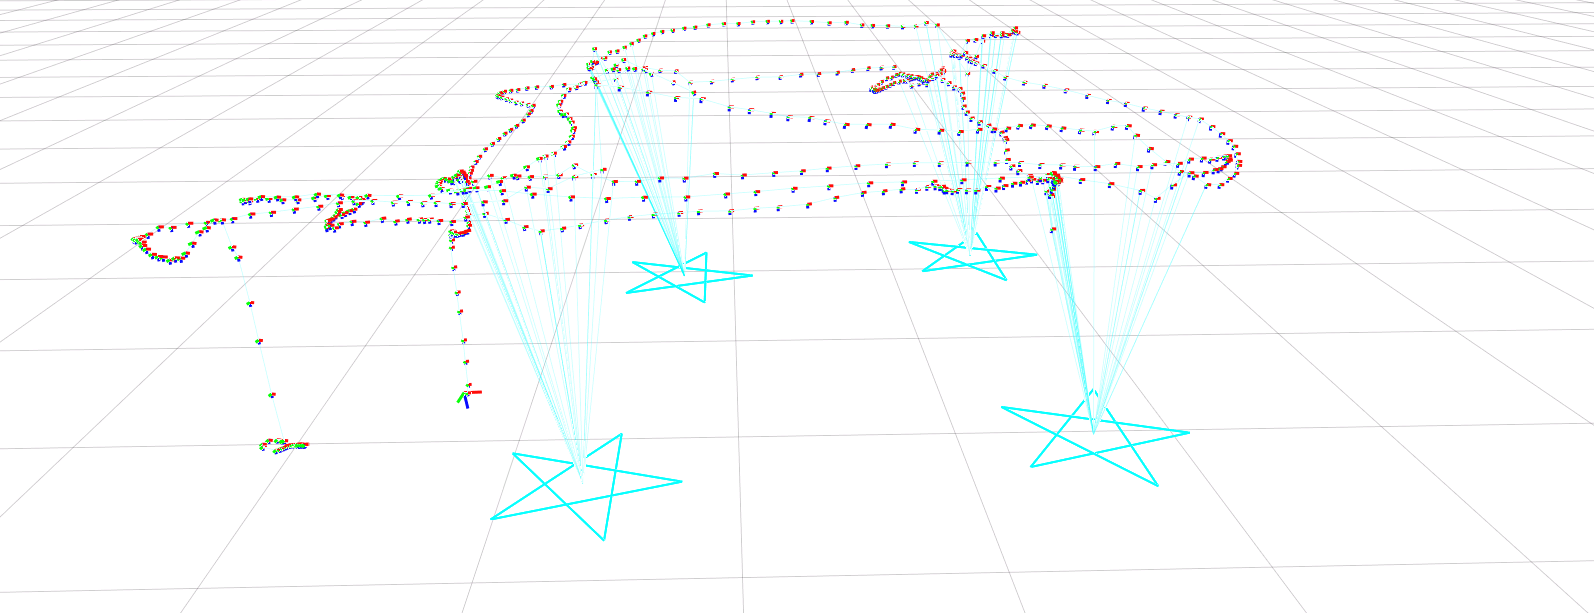
\includegraphics[width=1.0\textwidth]{images/square}
%    \caption{asdf}
%    \label{fig:square}
%  \end{center}
%\end{figure*}

\section{Parrot AR.Drone}
\label{sub:quadrotor}

% Steve talks about drone hardware
% Schuyler gets results

The quadrotor helicopter we used was a Parrot AR.Drone shown in Figure~\ref{fig:drone}.
Despite its reputation as an augmented reality gaming platform (for which it is
marketed), the AR.Drone has a substantial robotics community following. The AR.Drone has
a full suite of MEMS inertial sensors: a three-axis accelerometer, a two-axis gyroscope
for measuring pitch and roll, and a yaw angle precision gyroscope. It also features an
ultrasound altimeter and two cameras for recording images in the forward-looking and
downward-looking directions~\cite{ardronedevguide}.

\begin{figure}[!h]
  \centering
  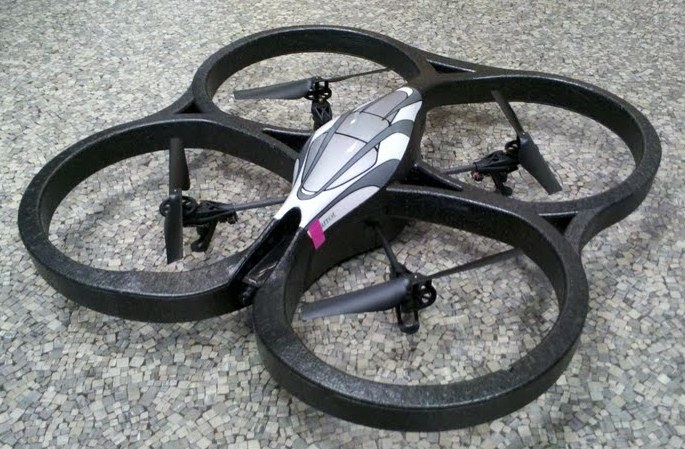
\includegraphics[width=2.5in]{images/drone1}
  \caption{The Parrot AR.Drone used for testing.}
  \label{fig:drone}
\end{figure}

The downward-looking camera was used to detect AprilTags acting as landmarks in our
environment. The AR.Drone itself fuses measurements from its inertial sensors and cameras
to provide estimates of velocities and Euler angles of the robot. The velocities reported
by the AR.Drone are not body-frame velocities, but rather velocities oriented with the yaw
angle of the body-frame and always parallel with the ground. The data available from the
AR.Drone that we used in our experiments is reported by a single LCM datatype. An overview
of this datatype is given in Table~\ref{tab:telemetry}.

\begin{table}[!t]
\renewcommand{\arraystretch}{1.3}
\caption{Telemetry from AR.Drone}
\label{tab:telemetry}
\centering
% BEGIN RECEIVE ORGTBL ardrone_state
\begin{tabular}{|l|l|}
\hline
Field & Description \\
\hline
Pitch & Euler angle about body-frame Y \\
Yaw & Euler angle about body-frame Z \\
Roll & Euler angle about body-frame X \\
Altitude & Height above ground \\
Vx & Forward velocity, parallel to the ground \\
Vy & Velocity to the right, parallel to the ground \\
Vz & Downward velocity, ground-perpendicular \\
Battery & Percentage of battery remaining \\
\hline
\end{tabular}
% END RECEIVE ORGTBL ardrone_state
\end{table}

\begin{comment}
#+ORGTBL: SEND ardrone_state orgtbl-to-latex :splice nil :skip 0
|----------+-----------------------------------------------|
| Field    | Description                                   |
|----------+-----------------------------------------------|
| Pitch    | Euler angle about body-frame Y                |
| Yaw      | Euler angle about body-frame Z                |
| Roll     | Euler angle about body-frame X                |
| Altitude | Height above ground                           |
| Vx       | Forward velocity, parallel to the ground      |
| Vy       | Velocity to the right, parallel to the ground |
| Vz       | Downward velocity, ground-perpendicular       |
| Battery  | Percentage of battery remaining               |
|----------+-----------------------------------------------|
\end{comment}

The front-end converts the measurements from the AR.Drone into relative poses (quadrotor
odometry). Both the camera images and state measurements are transmitted by the AR.Drone
over its own wireless ad-hoc network and passed into the front-end using LCM.


\section{Experiments}
\label{sec:experiments}

We applied our \ac{SLAM} implementation to simulated and real-world data. In both cases, we
evaluated batch least-squares \ac{SLAM}, incremental smoothing and mapping, and incremental
smoothing and mapping with variable reordering. 

\subsection{Simulation}
\label{sub:simulation}


To evaluate the speed of the three different methods, we used the simulator developed by
the University of Michigan APRIL lab. Before each test, we seeded the random number
generator to ensure the exact same data was being generated. The simulator represents a 2D
world, so we set the $z$ position, roll, and pitch observations to be zero with high
certainty. We chose to do this instead of using 2D nodes and factors to see the system
grow at the same rate of a full 6-\ac{DOF} application.

The three different methods of \ac{SLAM} that were evaluated had enormous speed
differences. Table \ref{tab:timing} shows the total simulation time for two loops of the
simulator which ensured that there were many loop closures.

\begin{table}[!t]
\renewcommand{\arraystretch}{1.3}
\caption{Total simulation time for different \ac{SLAM} methods}
\label{tab:timing}
\centering
\begin{tabular}{|c|c|}
\hline
Method & Total Simulation Time (s) \\
\hline
Incremental + Reorder & 18.81 \\
Incremental & 57.04 \\
Batch Solve & 912.96 \\
\hline
\end{tabular}
\end{table}

Figure \ref{fig:stepTime} shows the computation time spent at each update step for the
different methods. Notice the spikes at integer multiples of 100 for the incremental
methods. This is expected because it coincides with our batch update, optional variable
reordering, and relinearization. These results confirmed our suspicion that we would need
incremental updates as well as periodic variable reordering in order to achieve realtime
speeds when working with real-world data.

\begin{figure}[!t]
  \centering
  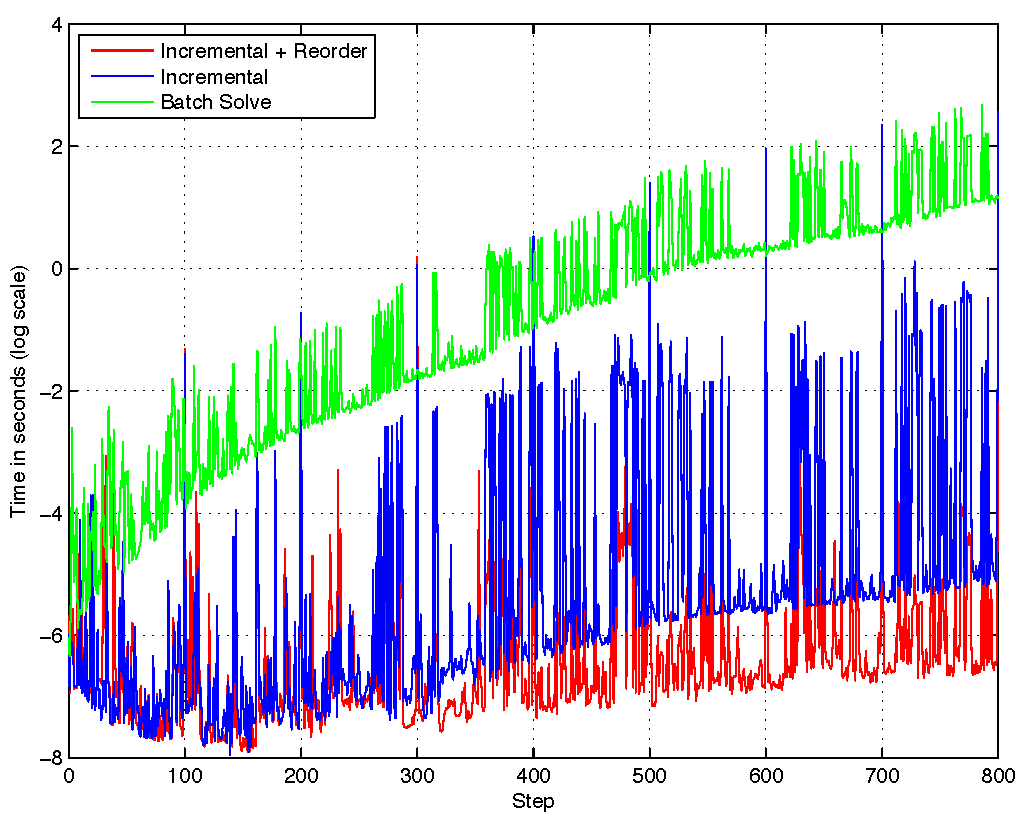
\includegraphics[width=2.5in]{images/stepTimeResults}
  \caption{The time per step for different \ac{SLAM} solve methods.  The incremental
    method with reordering (shown in red) is by far the fastest.}
  \label{fig:stepTime}
\end{figure}

We also ran our back-end on standard datasets to assess the computational performance and
accuracy of our implementation. For the Manhattan dataset~\cite{olson2006fast}, our final
normalized $\chi^2$ error value was 1.0399, which is comparable to that of iSAM's. On a
consumer grade computer, we finished the computations in 253 seconds. For the Victoria
Park dataset~\cite{Guivant00autonomousnavigation}, our final normalized $\chi^2$ error
value was 0.88614 and the total computation time was 489 seconds.
Figure~\ref{fig:manhattan} shows these results.

\begin{figure*}[!t]
  \begin{center}
    \subfigure[Manhattan dataset from~\cite{olson2006fast}] {
      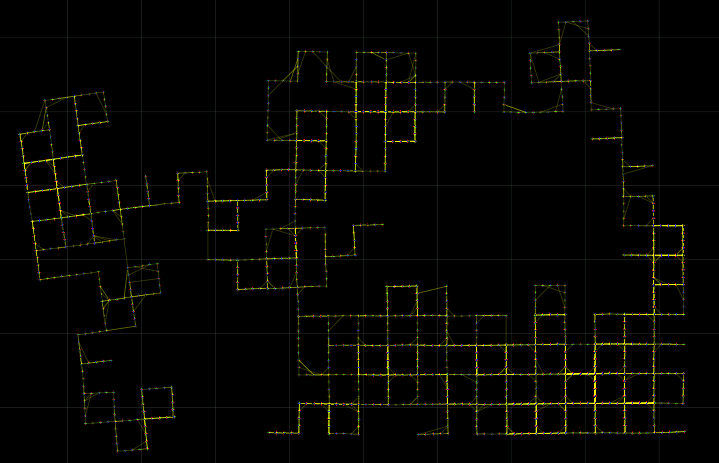
\includegraphics[width=3.0in]{images/manhattanOlson}
      \label{fig:manhattanResult}} \hspace{1cm}
    \subfigure[Manhattan World normalized $\chi^2$ error] {
      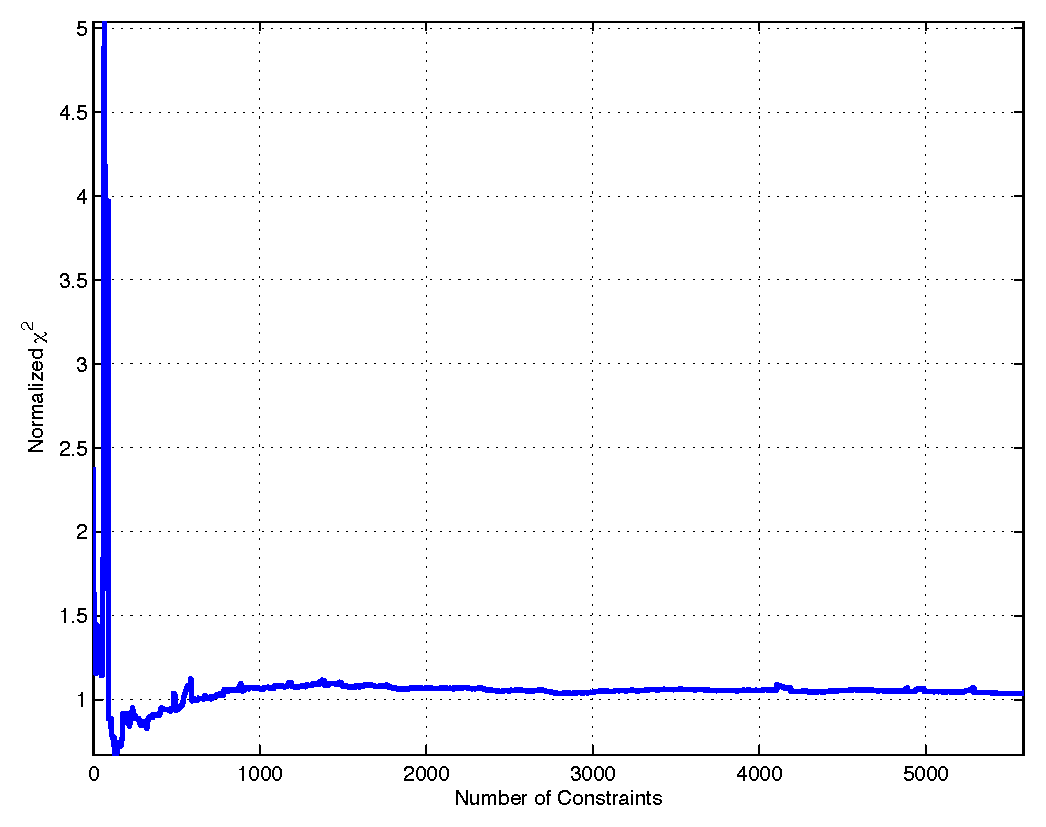
\includegraphics[width=2.5in]{images/chi2}
      \label{fig:manhattanChi2}}\\
    \subfigure[Victoria Park dataset from~\cite{Guivant00autonomousnavigation}] {
      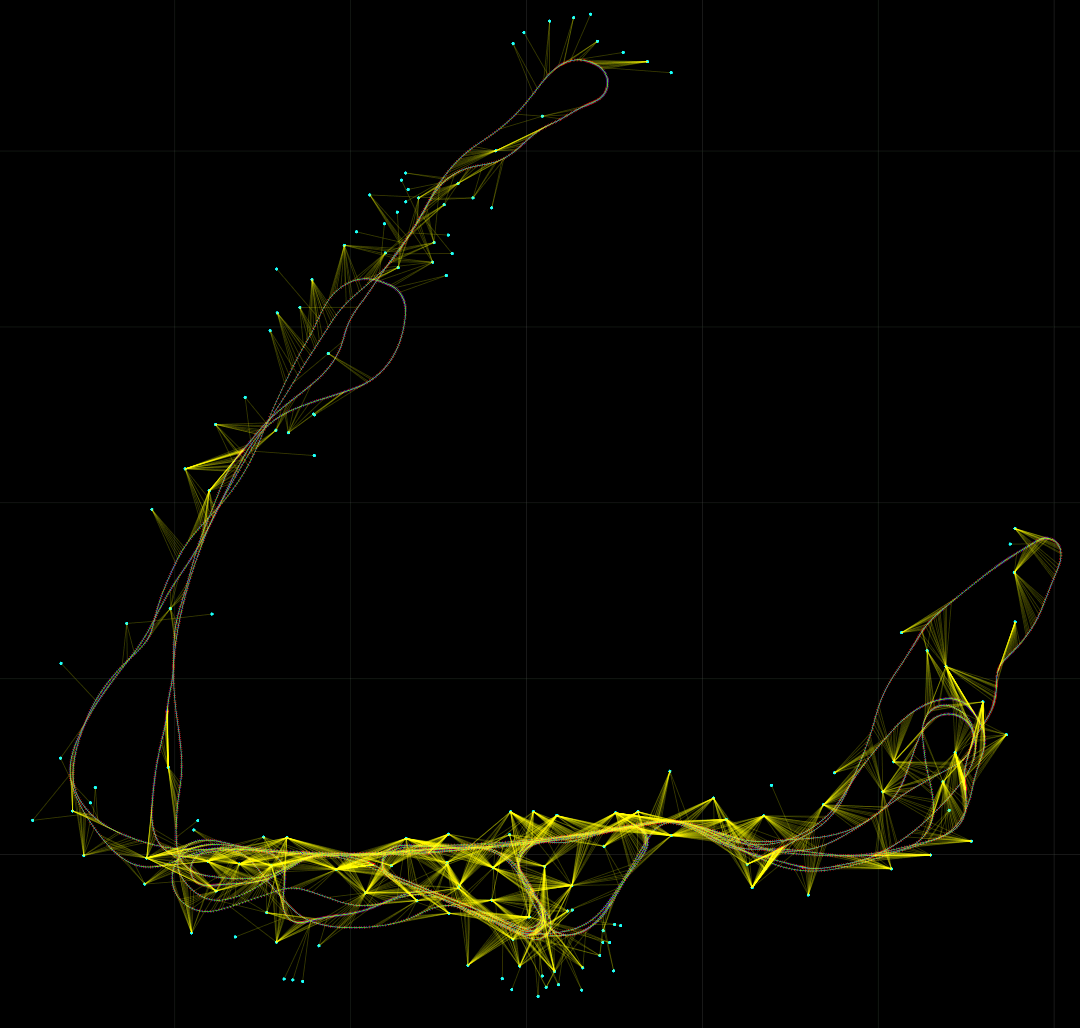
\includegraphics[width=3.0in]{images/victoriaPark}
      \label{fig:victoriaResult}} \hspace{1cm}
    \subfigure[Victoria Park normalized $\chi^2$ error] {\vspace{-5cm}
      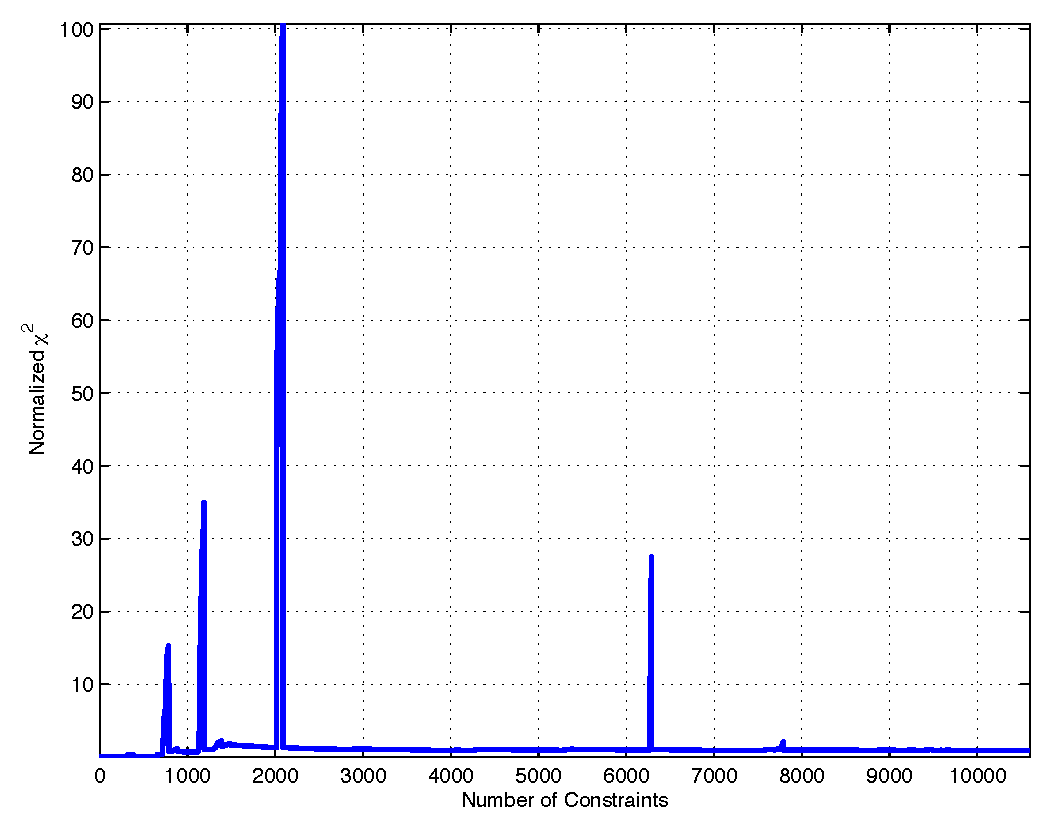
\includegraphics[width=2.5in]{images/chi2vic}
      \label{fig:victoriaChi2}}
  \end{center}
  \caption{As evidenced by the peaks in \subref{fig:manhattanChi2} and
    \subref{fig:victoriaChi2}, iSAM occasionally suffers from linearization errors. This
    is an inevitable consequence of the incremental update techniques. These errors are
    completely removed at the next batch step.}
  \label{fig:manhattan}
\end{figure*}


\subsection{Quadrotor Helicopter}
\label{sub:results}

\begin{figure*}[t]
  \begin{center}
    \subfigure[Experimental test run with four landmarks] {
      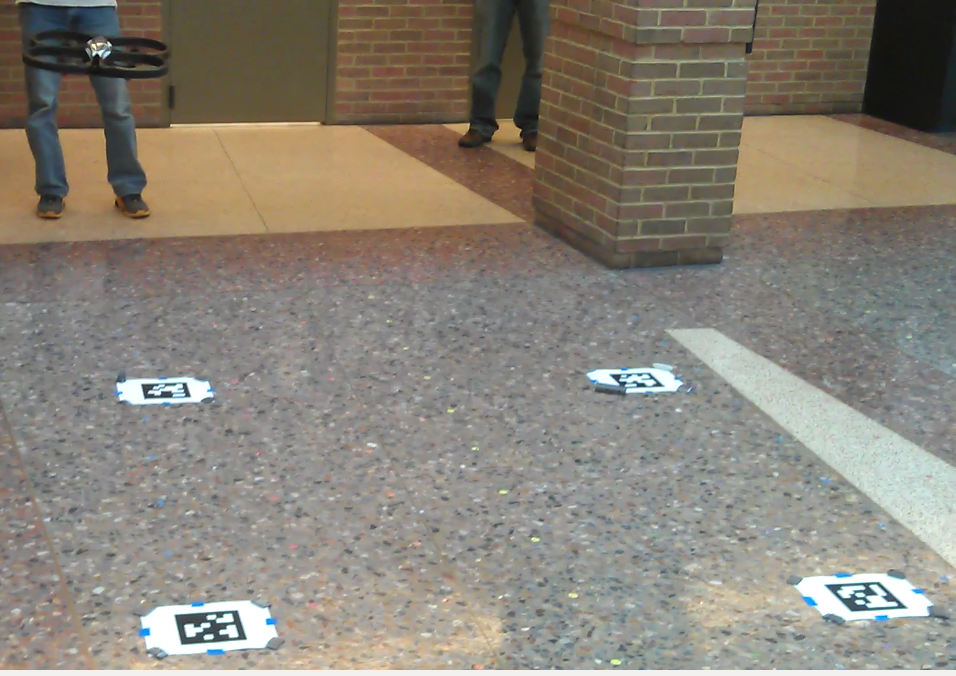
\includegraphics[width=2.1in]{images/setup}
      \label{fig:testing}}
    \subfigure[Dead reckoning] {
      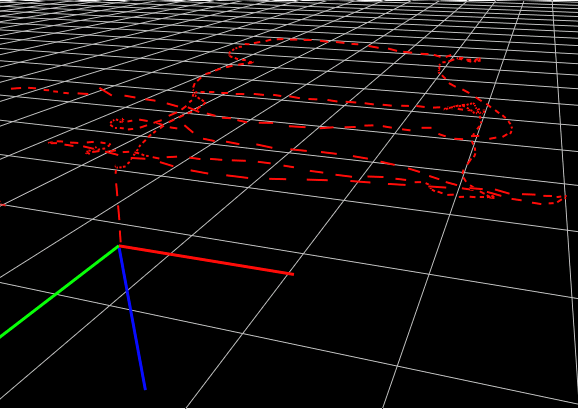
\includegraphics[width=2.1in]{images/deadreckon}
      \label{fig:deadreckon}}
    \subfigure[After closing the primary loop] {
      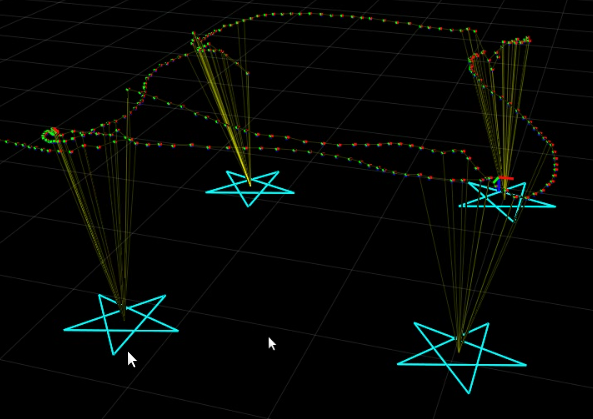
\includegraphics[width=2.1in]{images/loopclosure}
      \label{fig:loopclosure}}
    \caption{The map of the world created by the AR.Drone quadrotor with landmarks
      arranged in square.  In \subref{fig:deadreckon} the dead reckoning trajectory has
      significant drift in the $z$ direction (up/down).  This drift is corrected when
      using our \ac{SLAM} implementation~\subref{fig:loopclosure}.}
    \label{fig:mapadjustment}
  \end{center}
\end{figure*}

By arranging the landmarks in a known orientation, and flying the AR.Drone in a set
pattern, we were able to qualitatively evaluate the results of our experiments. Our
approach was to arrange 4 landmarks in a square and fly the AR.Drone around each edge
twice to gather loop closures. Since we did not use any ground-truth mechanisms, flying in
a square allowed us to evaluate the quality of our created map. A picture of one of our
test runs can be seen in Figure \ref{fig:testing}.

Our implementation was able to run and process data in realtime, providing a map that is
qualitatively acceptable.  As expected, the back-end corrects for drifts in the robot's
odometry, shown in Figures~\ref{fig:deadreckon} and \ref{fig:loopclosure}.

% As we run batch steps we see the map reorient itself into a better configurations as we
% gather more loop closures, as seen in Figure \ref{fig:loopclosure}. These results hold for
% any configuration of arbitrarily placed landmarks; simple shapes are used purely for ease
% of evaluation. Additionally, the path of the AR.Drone is significantly better than using
% dead-reckoning based off of the reported odometry, shown in Figure \ref{fig:deadreckon}.
% This is expected, as the position of the AR.Drone is calculated by double integrating
% accelerations, which can easily accumulate error and diverge over time.

Without knowing the ground-truth trajectory, absolute error in odometry and landmark
positions are impossible to calculate.  Therefore, we used normalized $\chi^2$ to
quantitatively evaluate the map produced by \ac{SLAM}.  After running on a nominal data
set, we find a final normalized $\chi^2$ error of 0.9719.  Because the expected
value of a normalized $\chi^2$ is 1, our solution is probabilistically reasonable.

One test run of the AR.Drone took about 60 seconds and produced about 1000 updates. We
were able to do all data gathering (reading and publishing LCM messages), pre-processing
(video decoding and AprilTag homography), and \ac{SLAM} solving using a personal laptop
with standard specs in realtime.

\section{Interactive Demonstration}

To interactively demonstrate our \ac{SLAM} back-end, we used a consumer-grade webcam
tracking a pre-assigned AprilTag to simulate odometry. Five other unique tags acting as
positional landmarks were added to the scene and tracked from a camera being moved by a
participant. A screen-capture of the program is shown in Figure~\ref{fig:interactiveDemo}.

This setup visually explained weighted least-squares in the context of \ac{SLAM}.  The
user could induce residuals for certain poses by physically moving a tag once the map has
been built.  The back-end optimized the graph and displayed it in realtime.  Watching this
unfold in a 3D scene proved to be a creative visualization of the problem,
especially for students who may not be familiar with least-squares SLAM.

\begin{figure}[h]
  \centering
  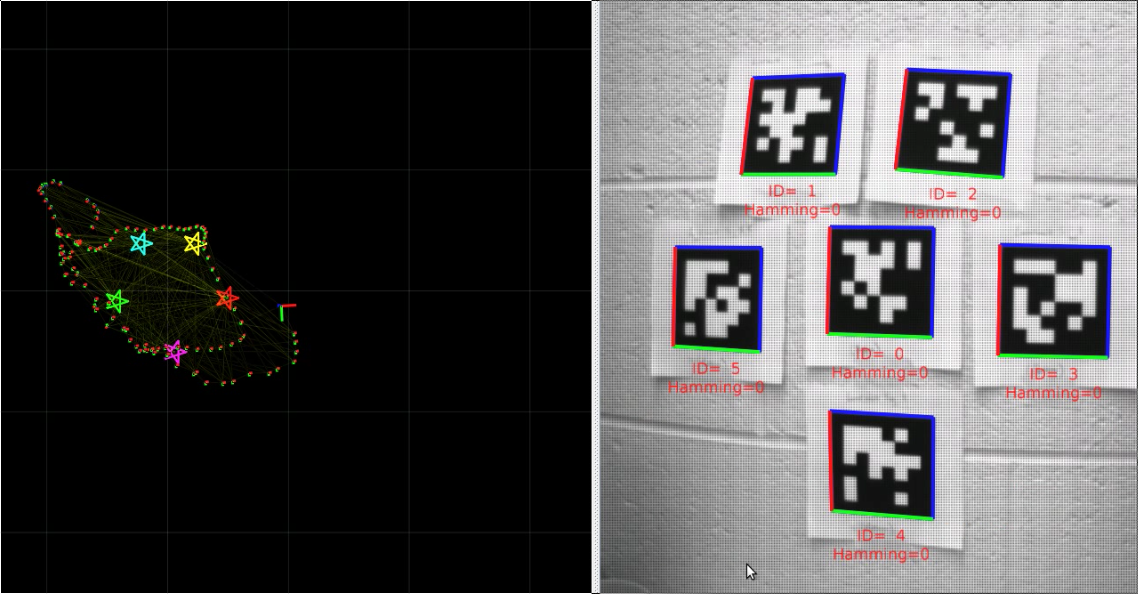
\includegraphics[width=3.0in]{images/interactiveDemo}
  \caption{A screen-capture of our table-top interactive
    demonstration.  The center tag provided us with simulated odometry
  and the remaining tags acted as landmarks.}
  \label{fig:interactiveDemo}
\end{figure}

\section{Conclusion}
\label{sec:conclusion}

% Schuyler's section
We have presented the development of an optimized, generic back-end solver for a 6-\ac{DOF}
\ac{SLAM} problem which is fast enough to allow for realtime deployment on a standard
computer.  Realtime operation was accomplished by using techniques from iSAM. We have 
deployed it in a real-world 6-\ac{DOF} application using known data
association with acceptable quality and $\chi^2$ error.


\bibliographystyle{IEEEtran}
% argument is your BibTeX string definitions and bibliography database(s)
\bibliography{IEEEabrv,references}


\end{document}



% An example of a floating table. Note that, for IEEE style tables, the
% \caption command should come BEFORE the table. Table text will default to
% \footnotesize as IEEE normally uses this smaller font for tables.
% The \label must come after \caption as always.
%
% \begin{table}[!t]
%%   increase table row spacing, adjust to taste
%   \renewcommand{\arraystretch}{1.3}
%   if using array.sty, it might be a good idea to tweak the value of
%   \extrarowheight as needed to properly center the text within the cells
%   \caption{An Example of a Table}
%   \label{table_example}
%   \centering
%%   Some packages, such as MDW tools, offer better commands for making tables
%%   than the plain LaTeX2e tabular which is used here.
%   \begin{tabular}{|c||c|}
%     \hline
%     One & Two\\
%     \hline
%     Three & Four\\
%     \hline
%   \end{tabular}
% \end{table}
